\documentclass[a4paper,10pt,twoside]{article}

%===========PACOTES
\usepackage[body={167mm,245mm}]{geometry}
%\usepackage[portuguese]{babel}
\usepackage{a1}
\usepackage[english]{babel}
\usepackage[latin1]{inputenc} %permite o uso de acentos
%\usepackage[dvips]{color}
\usepackage{amsfonts,amssymb}
%\usepackage{epsfig}
\usepackage{amsmath}
\usepackage{graphicx}	

% makeidx
\usepackage{makeidx}
% make index
\makeindex
%\usepackage[pdftex]{graphicx}


\def\mapright#1#2#3{\smash{\mathop{\hbox to
#3{\rightarrowfill}}\limits^{#1}_{#2}}}

\def\mapleft#1#2#3{\smash{\mathop{\hbox to
#3{\leftarrowfill}}\limits^{#1}_{#2}}}

\def\mapright#1#2{\smash{\mathop{\hbox to 0.90cm{\rightarrowfill}}\limits^{#1}_{#2}}}
\def\mapleft#1#2{\smash{\mathop{\hbox to 0.90cm{\leftarrowfill}}\limits^{#1}_{#2}}}

\def\mapleftright#1#2{\smash{\mathop{\hbox to 0.80cm{\leftarrowfill \rightarrowfill}}\limits^{#1}_{#2}}}
\def\ext{\times \! \vrule depth0pt height5pt width0.35pt}

\def\H{\mathcal H}
\def\D{\mathcal D}
\def\B{\mathcal B}
\def\C{\mathbb C}
\def\R{\mathbb R}
\def\S{\mathbb S}
\def\U{\mathcal U}
\def\Z{\mathbb Z}

\title{A challenge to 3-manifold topologists
\footnote{2010 Mathematics Subject Classification: 
57M25 and 57Q15 (primary), 57M27 and 57M15 (secondary)}} 
\author{Lauro D. Lins and S�stenes L. Lins}

\date{\today}


\begin{document}


\maketitle

\begin{abstract}
This paper is an instance of a very specific problem in 3-manifold topology.
``Important though the general concepts and propositions may be with the 
modern industrious passion
for axiomatizing and generalizing has presented us \ldots nevertheless I am convinced that
the special problems in all their complexity constitute the stock and the core of mathematics; 
and to master their difficulty requires on the whole the harder labor.'' Hermann Weyl 1885-1955, 
cited in the preface of the first edition (1939) of \cite{whitehead1997}.
\end{abstract}

\section{The first of various doubts in the classification of 3-manifolds}

The objective of this short note is to pinpoint an aspect of the classification of 
3-manifolds which is very important and has been essentially neglected in
the last three decades of success leaded by the works of W. Thurston, G. Perelman,
I. Agol and many others.
In despite of enormous progress, the 
classification problem remains, to our eyes, very difficult. The aspect we want to pinpoint is
questioning on hard to find tough instances of the general theory.

As an example consider the two closed 3-manifolds
obtained from surgery on the 2-component
framed links below. Both are homology spheres so their fundamental groups are perfect.
Snappea \cite{weeks2001snappea} tell us that they are both hyperbolic and have the same
volume. Moreover, their Witten-Reshetiken-Turaev invariants with 10 decimal places 
agree up to $r=12$. These facts seems to imply that the manifolds are homeomorphic.
However, computations based on techniques of 
\cite{lins2007blink} and \cite{lins1995gca}, which were up to this point successful
in finding homeomorphism between 3-manifolds, seems to fail for the first time.
Our bet is that the methodology does not fail: the manifolds are not homeomorphic.
In the last 5 years we have asked the help of 
various distinguished topologists in trying to settle
this example. None of them succeeded in answering our question. So,
we believe the time is ripe to bring our doubt to the whole community of matematicians
interested in 3-manifolds.

Being hyperbolic
replaces the difficult topological question of homeomorphism between the manifolds
into the possibly equality difficult algebraic question of
isomorphism between their fundamental groups. So, as long as the general associated
question is not settled,
we have replaced a problem which we do not know how to solve into another,
which we also do not know how to solve. This might be a wonderful 
progress, but hardly a definitive one.
In general, how to prove that the fundamental groups of hyperbolic 3-manifolds
are not isomorphic? Start by proving that there is no isomorphism between the 
fundamental groups of the 3-manifolds below. Or find one.


%-----------------------------------
\begin{figure}[!htb]
\begin{center}
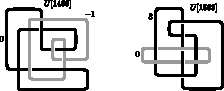
\includegraphics[scale=2.5]{A.figs/firstdoubt.pdf}
\caption{Are these 3-manifolds homeomorphic or not?}
\label{fig:dualPL2}
\end{center}
\end{figure}
%-----------------------------------


%-----------------------------------
\bibliographystyle{plain}
%\bibliographystyle{is-alpha}
%\addcontentsline{toc}{bibliografia}{\MakeTextUppercase{Refer�ncias Bibliogr�ficas}}
%\bibliography{d:/slsl\3.DadosSostenes.35.ArtigosLivros.bibtexGoogleScholar/bibtexIndex.bib} % bib file is slsl.bib
%\bibliography{~/home/ricardo/Dropbox/35.ArtigosLivros.bibtexGoogleScholar/bibtexIndex.bib}
\bibliography{bibtexIndex.bib}
%\bibliography{slsl}

\vspace{10mm}
\begin{center}

\begin{tabular}{l}
Lauro D. Lins\\
AT\&T Labs Research \\
Florham Park \\
180 Park Avenue \\
Florham Park, NJ 07932 \\
USA\\
llins@research.att.com
\end{tabular}
\hspace{20mm}
\hspace{7mm}
\begin{tabular}{l}
   S\'ostenes L. Lins\\
   Centro de Inform\'atica, UFPE \\
   Av. Jornalista Anibal Fernades s/n\\
   Recife, PE 50740-560 \\
   Brazil\\
   sostenes@cin.ufpe.br
\end{tabular}
\hspace{20mm}
\hspace{7mm}
\end{center}


\end{document}

% \printindex
